\documentclass[12pt,a4paper,oneside]{ctexart}

\usepackage{amsmath,amsthm,amssymb,appendix,bm,graphicx,hyperref,mathrsfs}
\usepackage{geometry,pifont,ctex}
\usepackage{float}  % 图片位置设置
\usepackage{listings} % 插入代码块
\usepackage{color}


\usepackage{enumitem}
\setlist[itemize]{itemsep=1.6pt, topsep=4pt, parsep=0pt, partopsep=0pt} % itemize 行距

\newtheorem{theorem}{定理}[section]
\newtheorem{corollary}{推论}[theorem]
\newtheorem{lemma}[theorem]{引理}
\newtheorem{remark}{注}[theorem]
\theoremstyle{definition}
\newtheorem{definition}{定义}[section]

\geometry{left=2.54cm,right=2.54cm,top=3.18cm,bottom=3.18cm}
\linespread{1.5}




% 设置标题、作者、日期
\title{Generals 将军棋 \\   
        \large{—— 2023年春季学期《数字逻辑设计》课程项目文档}}
\author{
    陈鑫圣 \quad 周晋 \\
    \small{清华大学计算机科学与技术系} \\
    \small{\texttt{\{cxs21,zhoujin21\}@mails.tsinghua.edu.cn}}
}

\date{\kaishu{\today}}

\begin{document}
% 标题
\maketitle
\newpage
% 目录
\tableofcontents
\newpage
% 各个章节
\section{项目介绍}
\subsection{选题背景}
% 或者叫“选题来源”等

Generals(或译为“将军棋”)
\footnote{游戏链接:\href{https://generals.io/}{https://generals.io/}}
\footnote{开发者页面:\href{https://dev.generals.io/}{https://dev.generals.io/}}
是一款多人对战的实时战略游戏,玩家需要操控兵力,攻城略地,以占领他人王城为最终目标,基本规则简单,但内容不失丰富有趣,更能开发出多种不同的游戏策略。

这款游戏在信息奥赛选手等圈子内具有广泛的知名度,而我们的舍友正是其中的一名达到过世界第一的深度玩家。受他的影响,我们对此游戏产生了浓厚兴趣。考虑到其功能实现的可行性强,我们决定在项目中复现该游戏。




\subsection{游戏规则}

\subsubsection{游戏局面}

游戏在一张 $10\times 10$ 的棋盘上进行,每个格子至少有以下 2 种属性:归属方、格子类型。对于“格子类型”非“山地”的格子,它还有“兵力”属性。

\noindent \textbf{归属方}

归属方即为该格子的拥有者,可以为红方玩家、蓝方玩家或非玩家(下称“NPC”)。
\begin{itemize}
    \item 对于归属方为玩家的格子,其“格子类型”可以为下述的“空地”、“城市”或“王城”。
    \item 对于归属方为NPC的格子,其“格子类型”可以为下述的“空地”、“城市”或“山地”。
\end{itemize}


\noindent \textbf{格子类型}
\begin{itemize}
    \item 空地(普通格子):初始时兵力为 0且归属于NPC。每16回合,所有\textbf{归属于玩家}的空地的兵力+1;归属于NPC的城市的兵力不变。
    \item 城市:初始时兵力为0且属于NPC。每1回合,所有\textbf{归属于玩家}的城市的兵力+1;归属于NPC的城市的兵力不变。
    \item 山地:归属于NPC且没有兵力属性。所有山地格子游戏开始(初始棋局生成)时确定,并自始至终不可被进行任何操作。
    \item 王城:每个玩家有且仅有一个王城,这也是玩家初始占有的唯一格子。每1回合所有王城的兵力+1。当某方玩家的王城被占领(见下方 \ref{subsubsection:operate-rules}“操作规则”)时,该玩家出局,游戏结束。
\end{itemize}

所有格子的格子类型在游戏全过程中不发生改变。

\noindent \textbf{兵力}

“兵力”属性仅“格子类型”非“山地”的格子拥有。该属性是一个非负整数值。在初始时,每方玩家的王城的兵力为9,其它所有格子的兵力均为0。


\subsubsection{操作规则} \label{subsubsection:operate-rules}
双方轮流进行行棋操作。每次操作有一定的时间上限,若达到此上限后仍未行棋,视为放弃本次行棋机会(但在计算行棋次数以及回合数时仍计入)。双方各操作一次(包括超时),计为1回合。

\noindent \textbf{兵力转移机制}

在每次操作中(不妨称操作方为“我方”),可以选择一个我方格子(设该格子的兵力为$n$),将该格子的部分兵力(称为“派出兵力”,其值设为 $d$)转移到一个相邻格子(称为“目标格子”,设其兵力为 $m$)上。转移后,源格子的兵力变为 $n-d$,而目标格子的归属方和兵力依下确定:

\begin{itemize}
    \item 若目标格子归属于我方:目标格子的归属方不变,兵力变为 $m+d$。
    \item 若目标格子归属于对方:发生交战,若 $m < d$,则目标格子的归属方变为我方,兵力变为 $d-m$;否则目标格子的归属方仍为对方,兵力变为 $m-d$。 
    \item 若目标各自归属于 NPC 且非山地:目标格子的归属方变为我方,兵力变为 $d$。
    \item 若目标格子是山地:无法进行此操作。
\end{itemize}

其中,派出兵力 $d$ 可以为 $n-1$ 或 $\lfloor \dfrac{n}{2} \rfloor$,由操作方玩家决定。见第 \ref{subsubsection:operate-modes} 节。

% 【语法】有序列表
% \begin{enumerate}
%   \item 项目 1
%   \item 项目 2
%   \item 项目 3
% \end{enumerate}


\noindent \textbf{操作模式} \label{subsubsection:operate-modes}

玩家使用WASD移动光标,使用SPACE(空格)选中格子(仅可选中己方格子),进入行棋模式。在行棋模式下,玩家可对该格子进行操作,具体而言:按Z可以切换“全移模式”(派出兵力为 $n-1$,默认选择)和“半移模式”(派出兵力为 $\lfloor \dfrac{n}{2} \rfloor$),然后接着使用WASD选择出兵的目标格子。


\noindent \textbf{胜负判断}

当某方玩家的王城被占领时,该玩家出局,游戏结束。

\noindent \textbf{深度限制}

每方玩家有15秒时间进行操作,在剩余5秒时,倒计时数字变红;若超时,则跳过该次操作机会,直接转到对方进行操作。

游戏最多进行999回合,若到达最大回合,对比双方王城兵力,多者获胜;若兵力相同,判为平局。



\subsection{仓库链接}
本项目开发过程通过清华 Git 进行版本控制管理。

清华 Git 仓库链接:\href{https://git.tsinghua.edu.cn/digital-design-lab/2023-spring/digital-design-grp-13}{https://git.tsinghua.edu.cn/digital-design-lab/2023-spring/digital-design-grp-13}。最终版本为 master 分支上的版本。

\section{效果演示说明}
% 这部分计划写的内容:
% - 附上效果图
% - 如何操作(例如先按 reset 再按 start 可以随机产生初始棋局和先手玩家)

\subsection{实验板使用}\label{subsection:circuit-usage}
\begin{figure}[H]
    \centering
    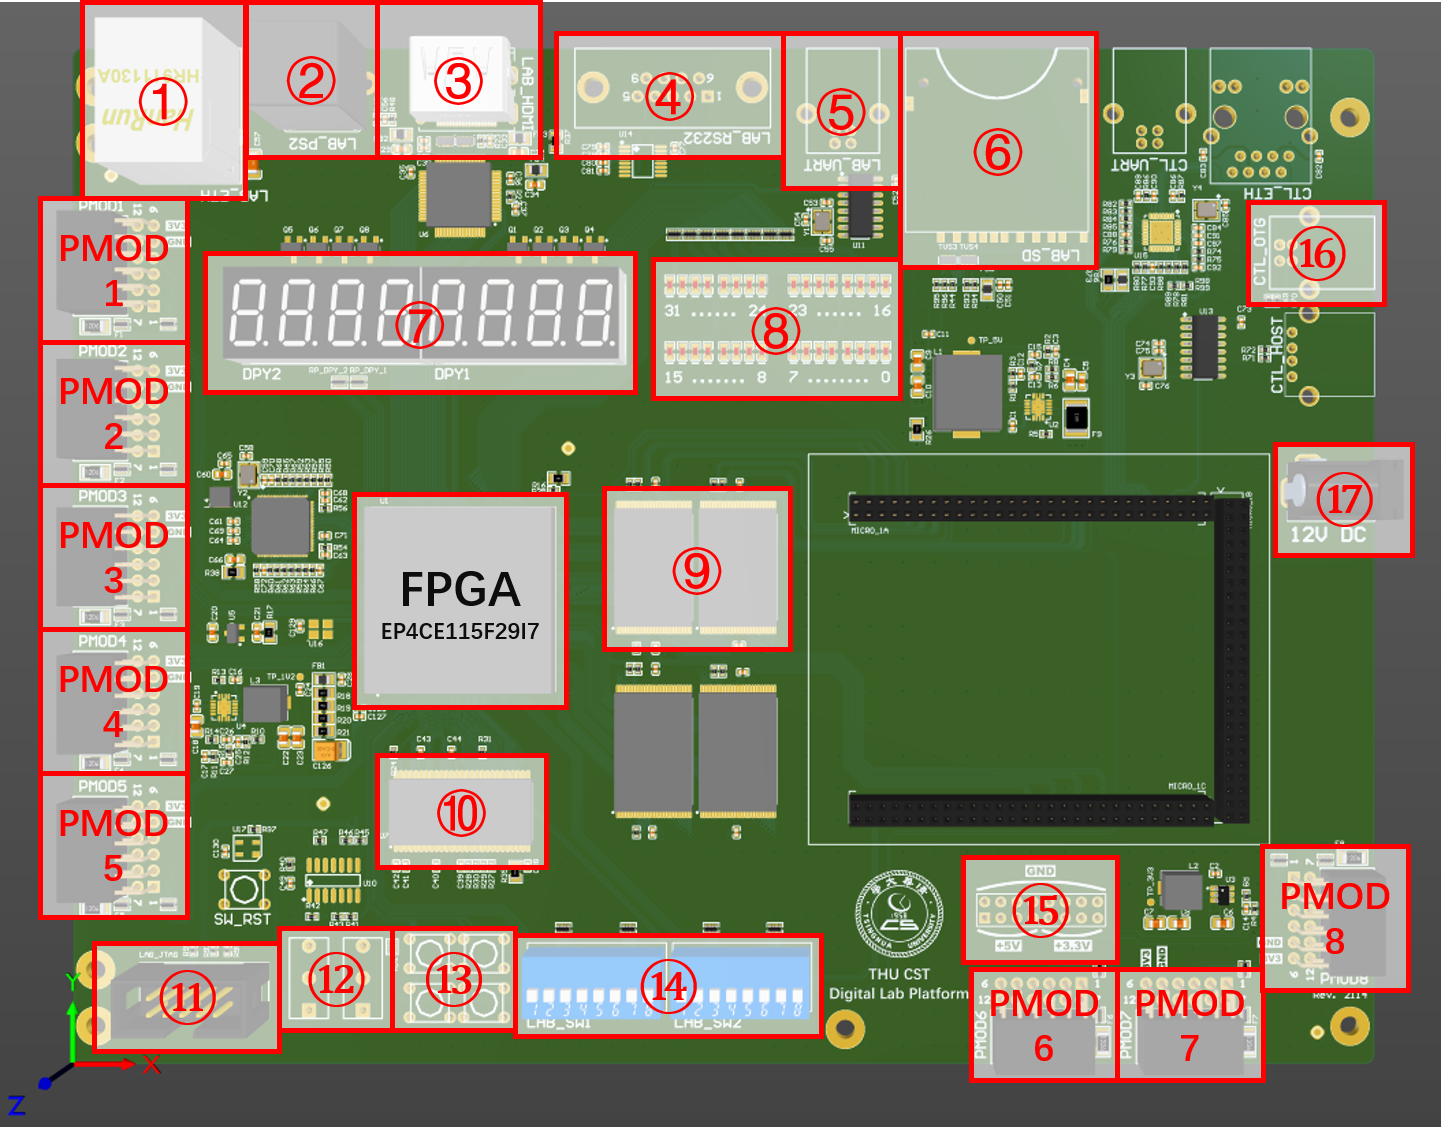
\includegraphics[scale=0.50]{images/board_anno.png}
    \caption{课程提供的实验板}
    \label{fig:board_anno}
\end{figure}

本项目在所给实验板上实现。使用的接口包括:
\begin{itemize}
    \item \textcircled{2}:PS/2接口,连接键盘;
    \item \textcircled{3}:HDMI接口,连接显示器;
    \item \textcircled{11}:FPGA JTAG调试接口,连接USB blaster,并接入电脑;
    \item \textcircled{12}去抖按键:用于开始游戏,生成随机初始棋局和随机先手玩家;
    \item \textcircled{17}电源:接入 12V 直流电源,用于给实验板供电。
\end{itemize}

\subsection{运行游戏}
在依第 \ref{subsection:circuit-usage} 节 连接好接口后,或者在需要重新开始一局游戏时,先按下“去抖按键”的左键(下称 reset 按钮),然后按下“去抖按键”的右键(下称 start 按钮),即可产生随机初始棋局和随机先手玩家,并自动开始游戏。

游戏开始后,玩家按第 \ref{subsubsection:operate-rules} 节(操作规则)所述方法进行操作。

\subsection{效果演示}

游戏效果演示视频见网络学堂提交的压缩包下的 \verb|doc/Videos| 文件夹。
\begin{figure}[H]
    \centering
    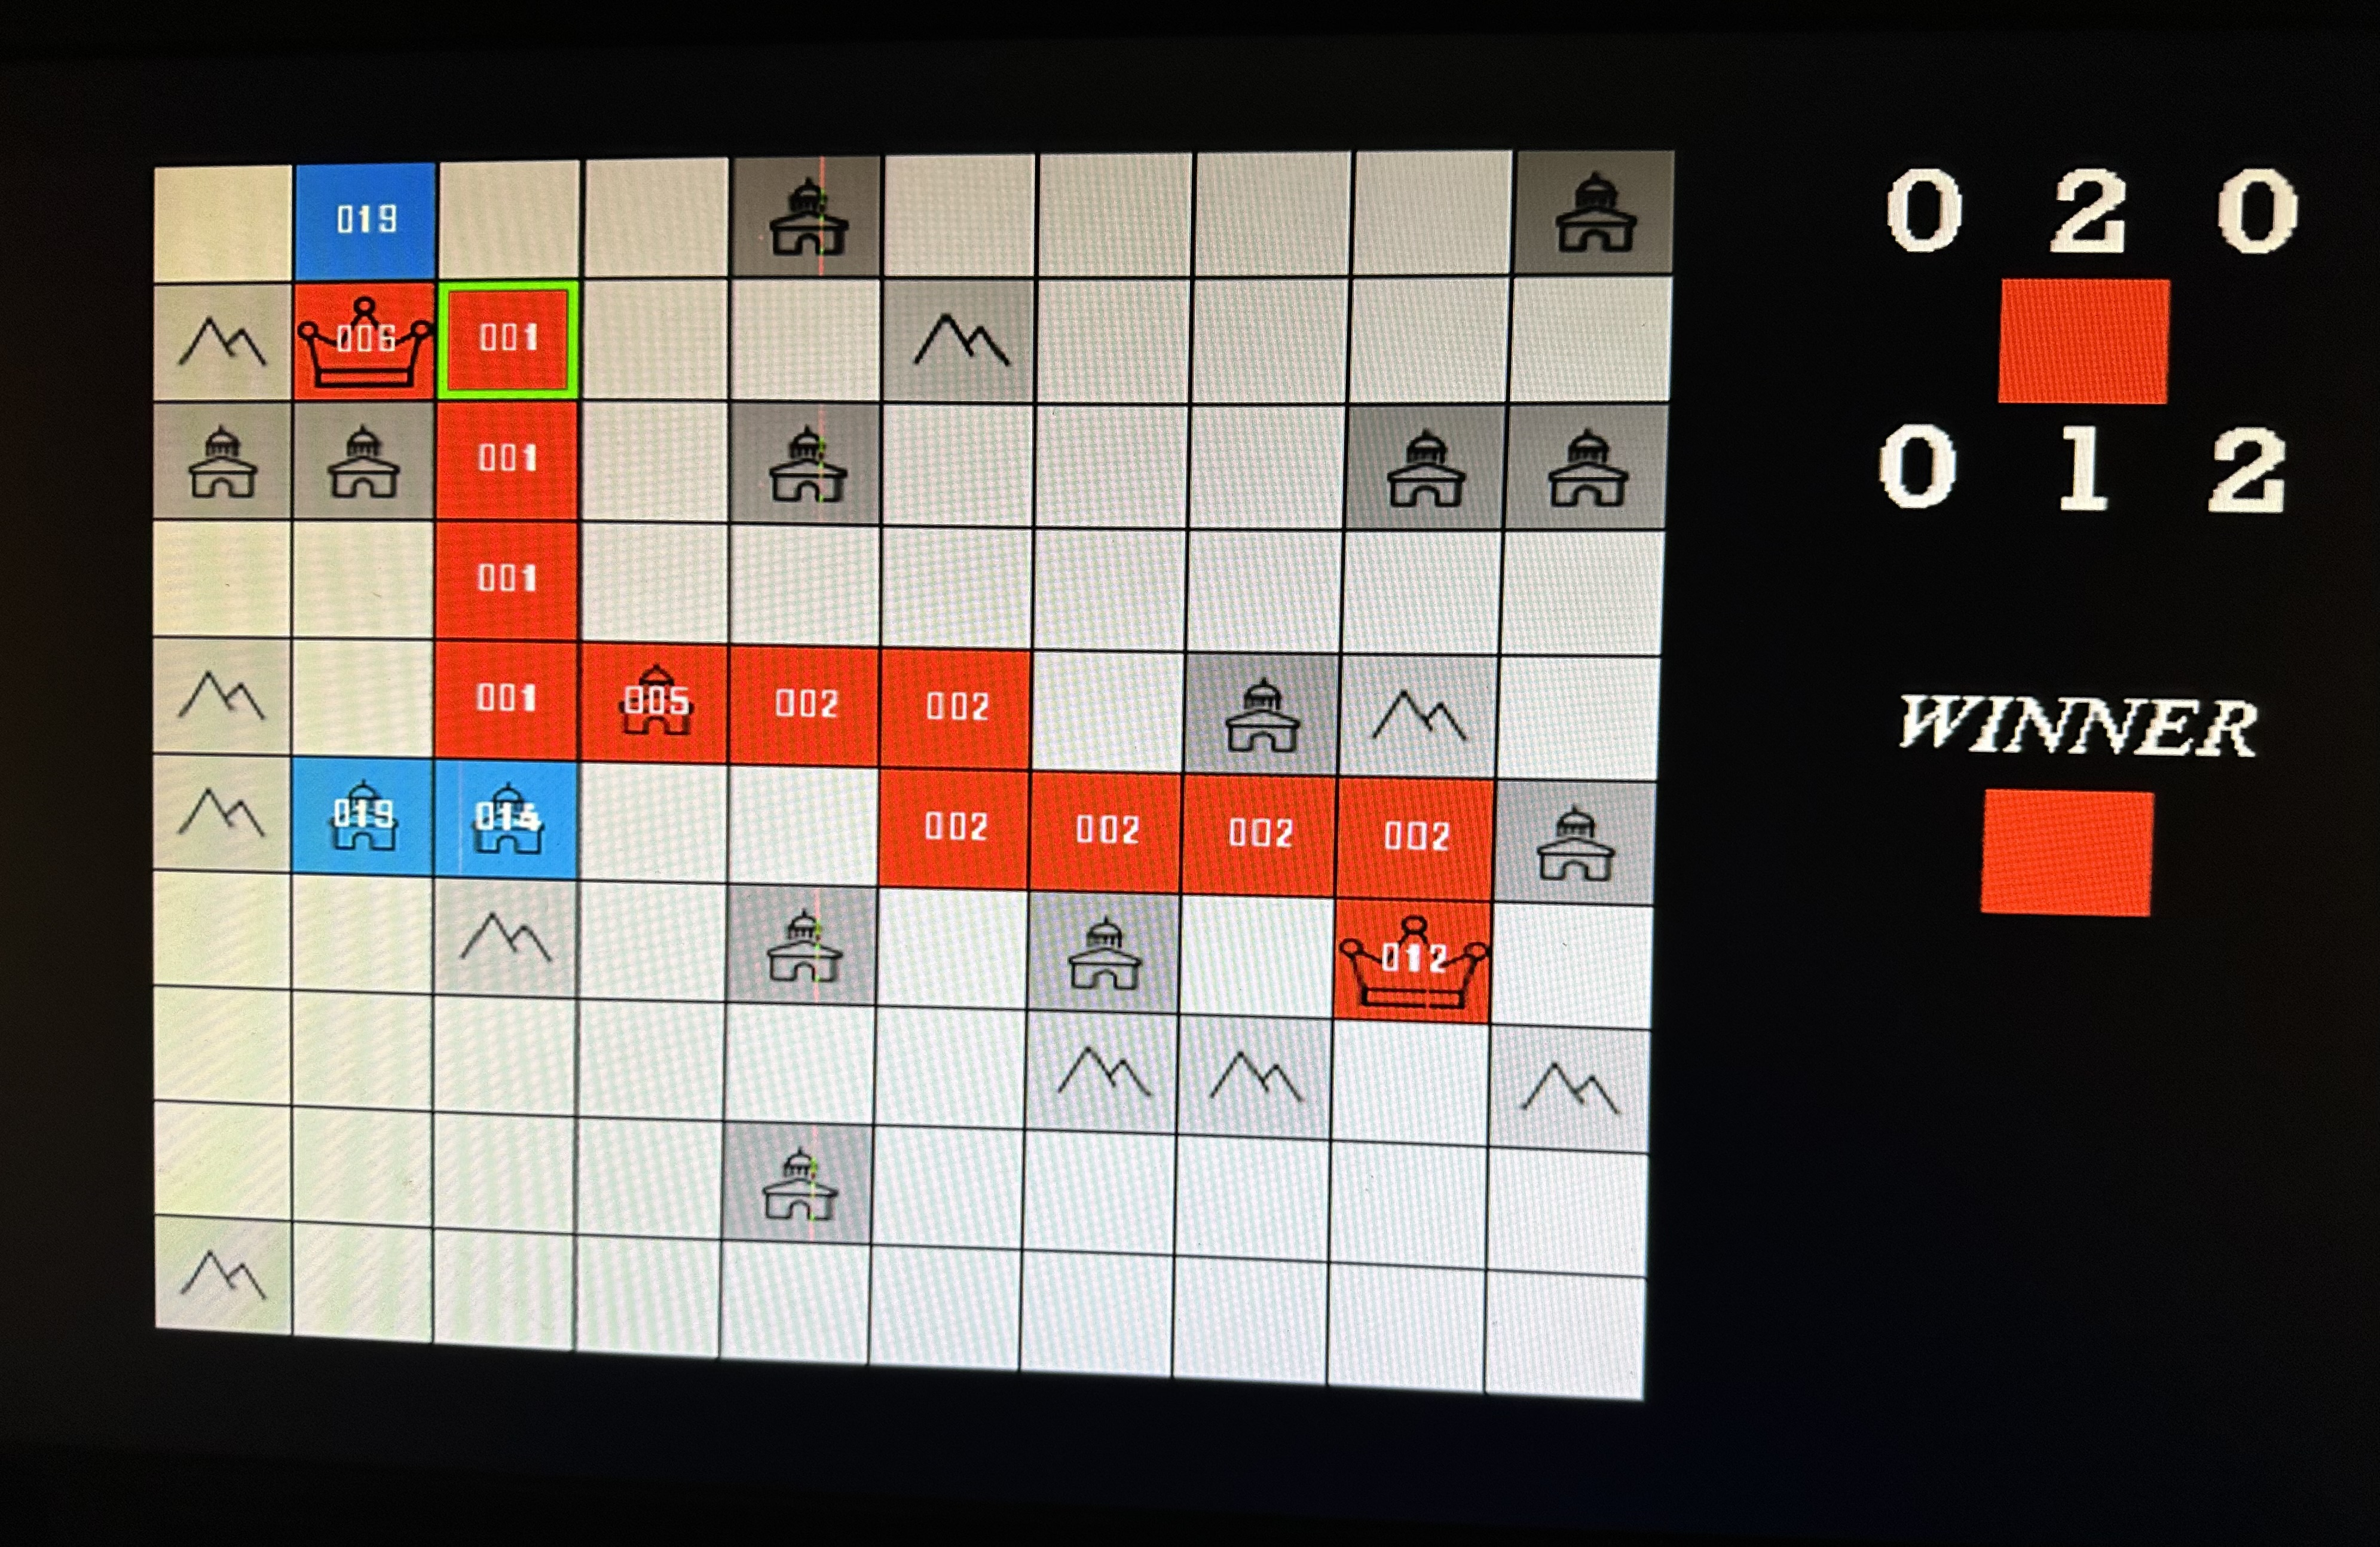
\includegraphics[scale=0.40]{images/demo.jpg}
    \caption{效果示例(红方胜利)}
    \label{fig:demo}
\end{figure}
\section{整体设计}
\subsection{模块划分} 
% 或者叫 “整体框架” 之类的?
整体结构图如下。

\begin{figure}[H]
    \centering
    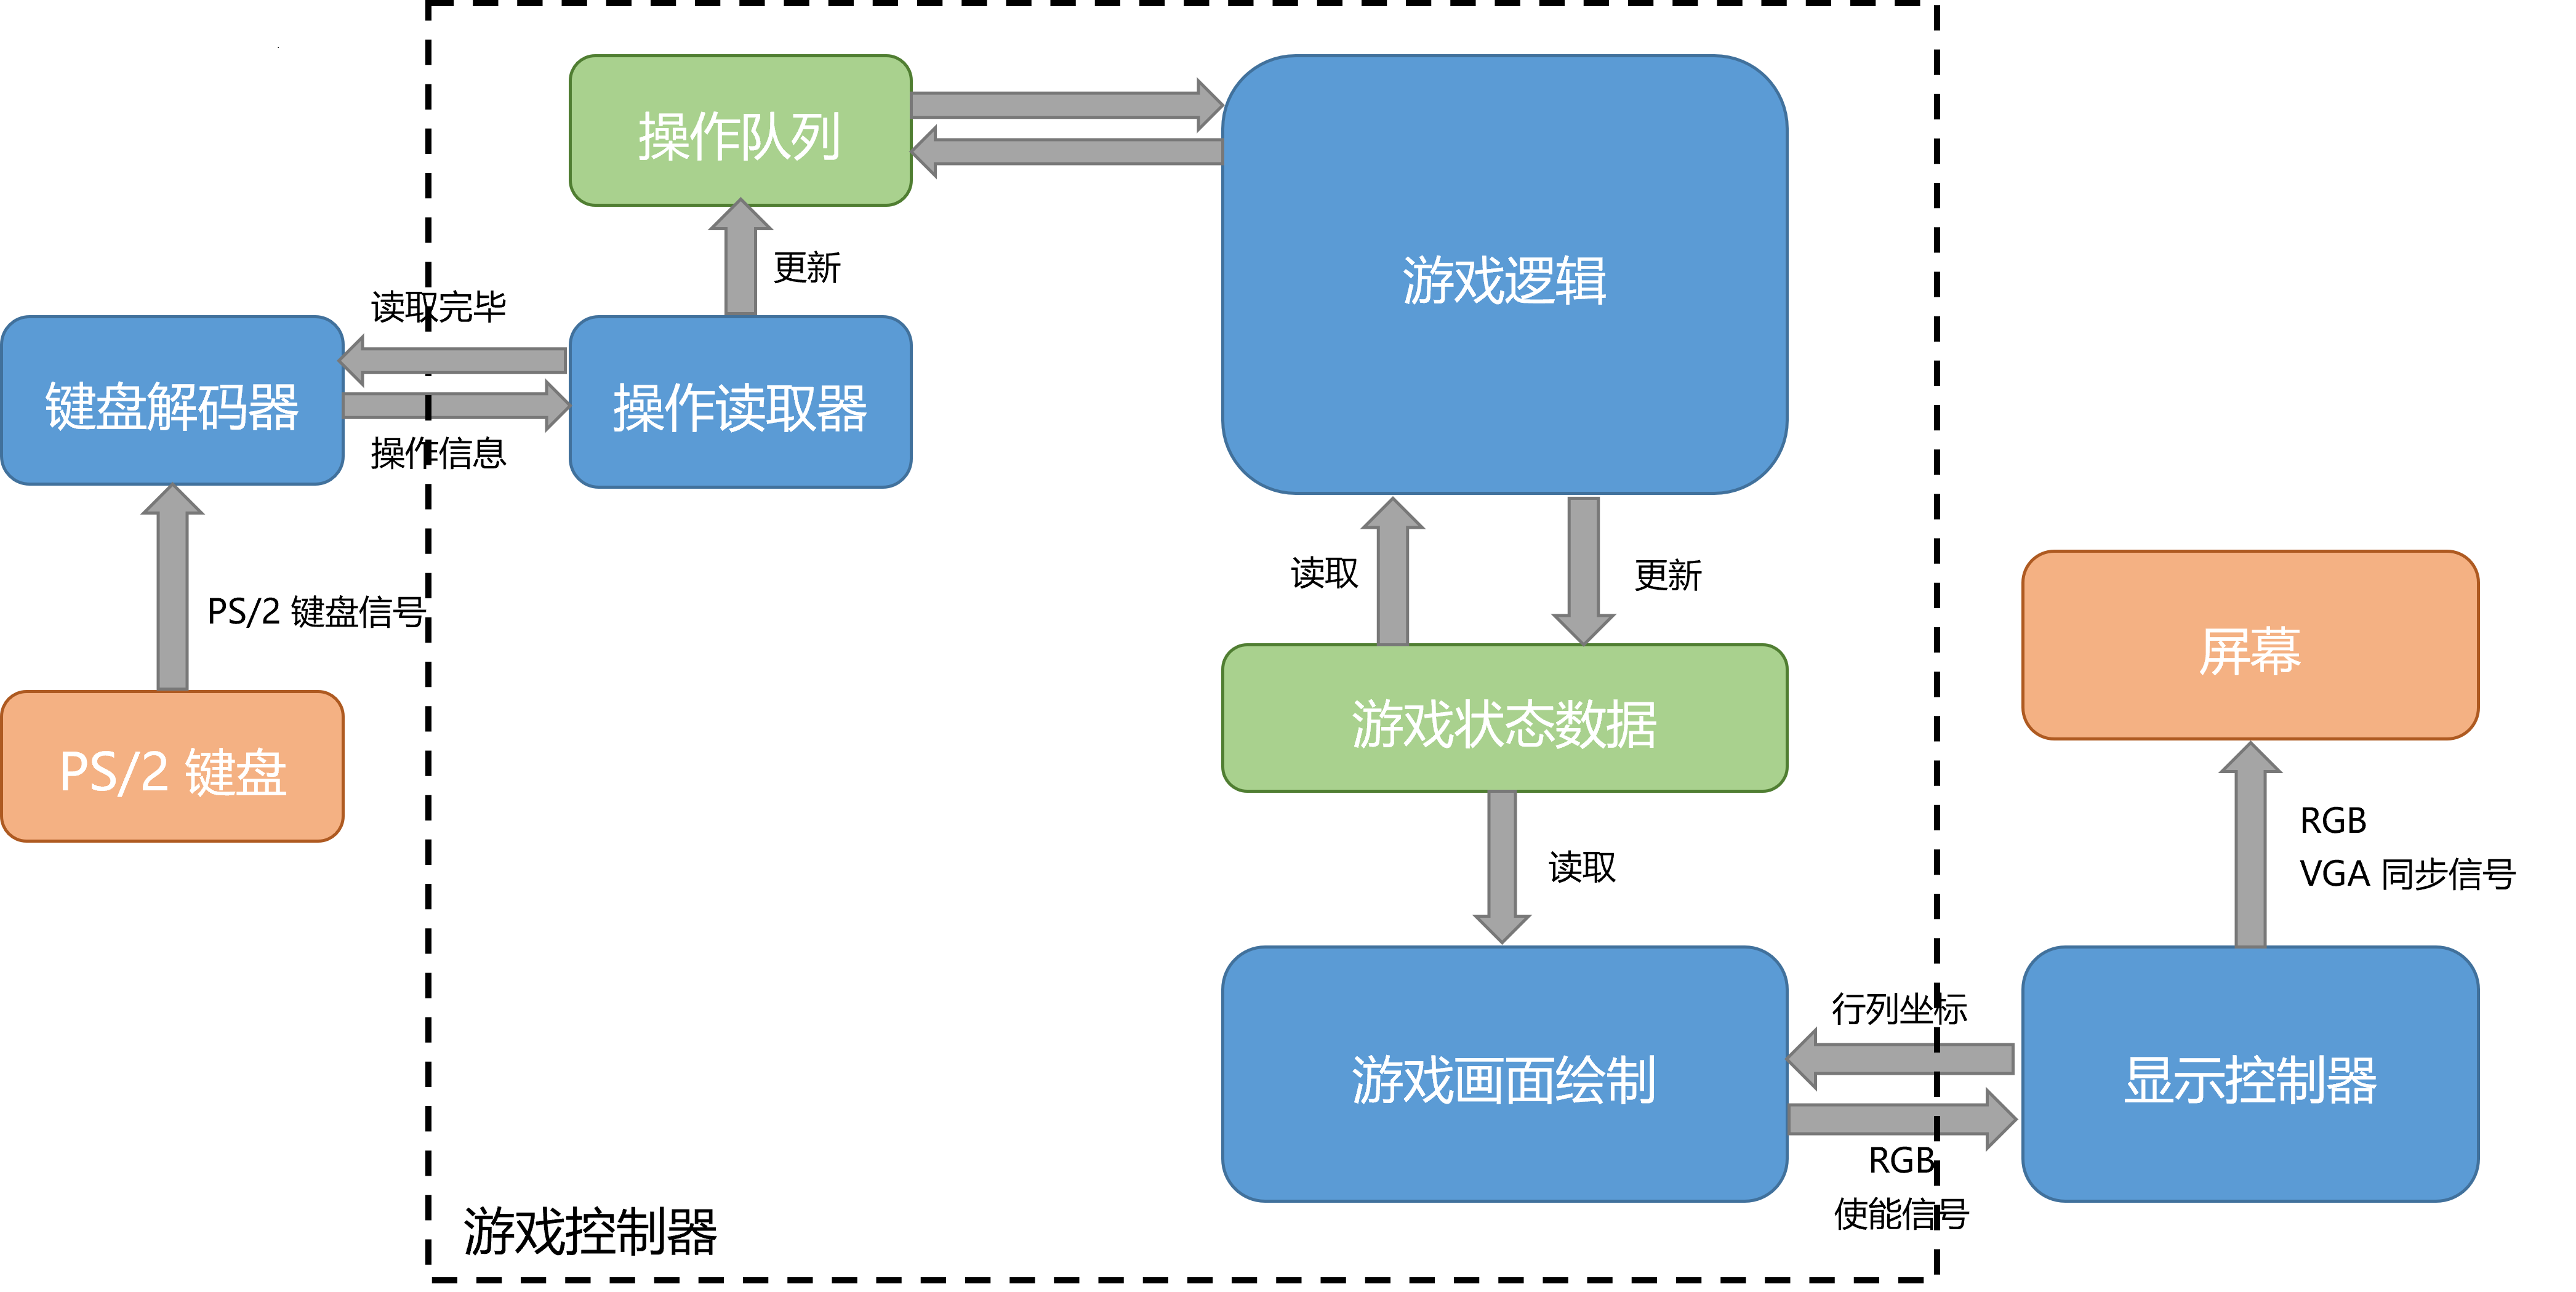
\includegraphics[scale=0.22]{images/structure.png}
    \caption{模块划分}
    \label{fig:structure}
\end{figure}

以上模块图中,橙色框表示外部设备,包括键盘,用以读取玩家的操作;VGA 显示器,用以输出游戏画面。蓝色框表示游戏中的计算和控制模块,包括和外部设备进行交互的键盘解码器和显示控制器,以及处理游戏内部逻辑的其它各模块(整体称为“游戏控制器”)。绿色框表示游戏内部维护的信息。

% 简要介绍各个模块的功能
\textbf{键盘解码器}使用一个状态机,接收并处理PS/2键盘发送的信号(断码),并将对应的操作信息传递给下游的操作读取器。

\textbf{操作读取器}是游戏控制器的上游部分,它读取来自键盘解码器的键盘操作信息,并将此信息写入操作队列(操作队列由操作读取器和游戏控制器共同维护)。

\textbf{游戏逻辑}是游戏控制器的核心部分。它内部用一个状态机维护游戏当前状态。在游戏即将开始时,它产生随机初始棋局和随机先手玩家。在游戏进行中,它从操作队列的队首读取一次键盘的按下信号,并基于游戏状态数据进行相应的计算;完成计算后,对游戏状态数据进行相应修改。

\textbf{游戏画面绘制}基于游戏状态数据,以及下游的显示控制器传回的VGA行列同步信号,计算当前扫描的像素的RGB值并传递给显示控制器。同时,它还判断该像素应该显示棋局信息还是背景图像信息,并向显示控制器输出此信号(即使能信号)。

\textbf{显示控制器}是下游屏幕输出的控制模块。它产生VGA行列同步信号,并将此信号传递回游戏画面绘制部分,从游戏画面绘制部分得到与当前棋局对应的画面信息后,对棋局画面和背景画面进行数据选择,得到最终画面的RGB值。最后,显示控制器将VGA行列同步信号和最终画面的RGB值输出到屏幕。

\subsection{模块间交互信号}

\subsubsection{键盘解码器与游戏控制器} \label{subsubsection:interact-input-logic}

\textbf{从键盘解码器到游戏控制器}
\begin{itemize}
    \item \texttt{ready}:1 bit。1表示有新数据(识别到键盘断码),0表示暂无新数据
    \item \texttt{data}:3 bit。表示识别到的键(WASD、空格、Z)
\end{itemize}

\textbf{从游戏控制器到键盘解码器}
\begin{itemize}
    \item \texttt{read\_fin}:1 bit。1表示数据已经被读取,否则为 0。
\end{itemize}

\subsubsection{游戏控制器与显示控制器}

\textbf{从游戏控制器到显示控制器} \label{subsubsection:interact-logic-output}
\begin{itemize}
    \item \texttt{gen\_red}, \texttt{gen\_green}, \texttt{gen\_blue}:各 8 bit。表示基于游戏局面计算出的游戏画面信息。
    \item \texttt{use\_gen}:1 bit。表示当前像素是使用游戏逻辑生成的棋局图像(1)还是背景图像(0)
\end{itemize}

\textbf{从显示控制器到游戏控制器}
\begin{itemize}
    \item \texttt{hdata\_o}, \texttt{vdata\_o}:各 10 bit。表示当前扫描到的行列坐标。
\end{itemize}


\subsection{文件结构}
% 需要写出每个文件对应以上模块划分图中的哪些部分(模块)

本项目提交的压缩包中的 \verb|design/| 为实验的完整工程。\textbf{在该目录下}, \texttt{digital-design.sof} 为编译后的 bitstream 二进制文件;\texttt{src/} 目录下为源代码(ip 核除外)。

\texttt{src/} 目录下的文件如下(以下按对应模块的层次关系排列):

\begin{itemize}
    \item \texttt{mod\_top.sv} :项目的顶层文件
    \begin{itemize}
        \item \texttt{Keyboard\_Decoder.sv} :键盘解码器
        \item \texttt{Game\_Controller.sv} :游戏控制器
        \begin{itemize}
            \item \texttt{Counter.sv} :循环计数器,(计数频率较高时)可用于产生小范围内的伪随机数
            \item \texttt{Number\_Choose.sv} :用于显示数码
            \item \texttt{Number\_Transfer.sv} :用于计算一个三位数的百位、十位、个位
            \item \texttt{Random\_Boards\_Library.sv} :初始棋盘库,由 \texttt{random\_boards.py} 生成,用于随机选择初始棋盘
        \end{itemize}
        \item \texttt{Screen\_Controller.sv} :显示控制器
        \begin{itemize}
            \item \texttt{Background\_Painter.sv} :用于绘制背景图像
            \item \texttt{vga.v}: VGA 控制器,用于生成 VGA 行列扫描信号
        \end{itemize}
    \end{itemize}
\end{itemize}


\subsection{分工情况}

分工情况如下:
\begin{itemize}
    \item 总体架构设计:陈鑫圣
    \item 输入部分:周晋、陈鑫圣
    \item 游戏逻辑部分:陈鑫圣
    \item 输出部分:周晋
    \item 报告撰写:陈鑫圣、周晋
\end{itemize}
\section{各模块介绍}
% 每个模块需要写出对应的 module 的名字,从而和代码对应起来。
% 每个模块需要写其输入输出信号,以及部分关键的内部数据。

\subsection{键盘解码器与操作读取器} \label{subsection:keyboard-decoder}

\subsubsection{实现细节}
项目中与键盘解码器对应的 module 为 \texttt{Keyboard\_Decoder} (在文件 \texttt{Keyboard\_Decoder.sv} 中);与操作读取器对应的 module 为 \texttt{Game\_Controller} (在文件 \texttt{Game\_Controller.sv} 中)。

键盘解码器会接收所接键盘外设的断码(即松开时键盘传递的扫描码),并判断是否为需要的WASD Z SPACE按键,再进行编码,传给游戏控制器(中的操作读取器)。
% 编码方式如下:W A S D SPACE Z 依次编为 000 至 101。

为了保证每个键松开的信号被识别且仅被识别一次,两者会互相维护两个确认信号: \texttt{ready} 和 \texttt{read\_fin},分别表示有新数据和数据读取完成。

交互过程如下:
\begin{itemize}
  \item 当键盘解码器从键盘读取到按键断码时,将 \texttt{ready} 信号置为 1 ,并在将数据信号设定为相应的信息。
  \item 当游戏控制器接收的 \texttt{ready} 信号为 1 时,就读取数据,并将 \texttt{read\_fin} 信号置为 1。
  \item 当键盘解码器接收的 \texttt{read\_fin} 为 1 时,状态机在本次时钟周期不进行状态转移,并将 \texttt{ready} 信号恢复为 0。
  \item 当游戏控制器接收的 \texttt{ready} 信号为 0 时,就将 \texttt{read\_fin} 信号恢复为 0。至此,完成一次数据传递。
\end{itemize}

% 键盘模块读入\texttt{read\_fin}信号,在输出键盘信息的同时输出\texttt{ready}信号。\texttt{ready}信号默认为0,若\texttt{read\_fin}为0,且读入了合法的按键(即WASD Z SPACE),则\texttt{ready}信号为1,代表传入了新按键信息,传给游戏控制器,再将\texttt{ready}信号置为0。

% 主逻辑部分读入\texttt{ready}信号,并向键盘模块传入\texttt{read\_fin}信号;\texttt{read\_fin}信号默认为0,当接收到\texttt{ready}信号为1时,主逻辑开始读入传来的键盘数据,当读取完毕时,使\texttt{read\_fin}信号为1,传入键盘模块,再将\texttt{read\_fin}信号置为0。

\subsubsection{模块接口} \label{subsubsection:keyboard-decoder-interface}
下面为模块接口:
\begin{lstlisting}[
    language=Verilog,
    numbers=left,
    frame=single,           % 添加边框
    basicstyle=\fontsize{12}{12}\selectfont, % 设置全局字号
    lineskip=4pt,           % 设置行距
    tabsize=4,              % 设置制表符的宽度为4个空格
    xleftmargin=15pt,       % 设置左侧缩进的距离为15pt
    caption={\texttt{Background\_Painter}源代码} % 标题
] 
module Keyboard_Decoder (
    // input
    input wire          clock,
    input wire          reset,
    input wire          ps2_clock,   // PS/2 时钟信号
    input wire          ps2_data,    // PS/2 数据信号
    input wire          read_fin,    // 逻辑模块 -> 键盘输入
    模块的信号,1表示数据已经被读取
    // output
    output wire         ready,       // 键盘输入模块 -> 逻辑    
    模块的信号,1表示有新数据
    output wire [2: 0]  data         //输出,为WASD SPACE 
    Z编码后传入主逻辑
);
\end{lstlisting}
输入:
\begin{itemize}
    \item \texttt{ps2\_clock}:输入时钟,为$100M \text{Hz}$
    \item \texttt{ps2\_data}:键盘输入数据,为按下/松开键盘按键时传入的扫描码
    \item \texttt{read\_fin}:读取完成确认,由游戏控制器传入,1表示已读取,可以传递新数据,即把\texttt{ready}置为1
\end{itemize}
输出:
\begin{itemize}
    \item \texttt{ready}:传递新数据确认,当读取完成断码,且判断为需要的按键,且游戏控制器传来的完成确认为1时,置为1,表示要传递新数据
    \item \texttt{data}:传给游戏控制器的键盘数据,为需要的按键编码后传输,具体编码为:
    \begin{itemize}
        \item W:000
        \item A:001
        \item S:010
        \item D:011
        \item 空格:100
        \item Z:101
    \end{itemize}
\end{itemize}


\subsection{游戏控制器}
由于游戏逻辑部分和操作读取器需要共同维护操作队列,并且需要向下游的游戏画面绘制部分提供游戏状态数据,所以在实现中,我们将这三个部分以及“操作队列”“游戏状态数据”封装为“游戏控制器”(参见图 \ref{fig:structure} )。其中的操作读取器已在第 \ref{subsection:keyboard-decoder} 节介绍。

工程代码中对应的 module 为 \texttt{Game\_Controller} (在文件 \texttt{Game\_Controller.sv} 中)。

\subsubsection{游戏内部数据}

游戏控制器内部维护的数据如下:
\begin{itemize}
    \item 棋盘结构体数组:一个 $10\times 10$ 的二维数组,每一项是一个结构体(见下),表示一个格子的信息。
    \item 每个玩家王城的位置。
    \item 操作队列。在实现中,操作队列容量为 1,即只记录最近一次未被计算的操作。在实现中用一个3 bit 的寄存器来表示,在 \ref{subsubsection:keyboard-decoder-interface} 的基础上,增加“空队列” NONE(110)
    \item 当前玩家
    \item 当前光标位置
    \item 光标所处模式:光标移动模式(00 与 01),行棋模式(全移模式:10,半移模式:11)
    \item 已经进行的行棋操作次数(包括超时)
    \item 当前回合(从 1 开始)
    \item 当前游戏状态
    \item 当前回合剩余时间
\end{itemize}

每个单元格结构体定义如下:
\begin{lstlisting}[
    language=Verilog,
    numbers=left,
    frame=single,           % 添加边框
    basicstyle=\fontsize{10}{12}\selectfont, % 设置全局字号
    lineskip=4pt,           % 设置行距
    tabsize=4,              % 设置制表符的宽度为4个空格
    xleftmargin=15pt,       % 设置左侧缩进的距离为15pt
    % firstnumber=59,
    caption={单元格结构体} % 标题
] 
// 玩家类型
typedef enum logic [LOG2_MAX_PLAYER_CNT - 1:0]  {NPC, RED, BLUE} Player;
// 棋子类型
typedef enum logic [LOG2_PIECE_TYPE_CNT - 1:0]  
    {TERRITORY,              MOUNTAIN,    CROWN,   CITY      } Piece;
    // 普通领地(含空白格), 山,         王城,    塔(城市)
// 单元格结构体
typedef struct packed {
    Player                        owner;        // 该格子归属方
    Piece                         piece_type;   // 该棋子类型
    reg [LOG2_MAX_TROOP - 1: 0]   troop;        // 该格子兵力值
} Cell;
\end{lstlisting}

\subsubsection{游戏状态机}
在游戏逻辑部分,用一个状态机来维护游戏内部状态。各状态定义如下:
\begin{lstlisting}[
    language=Verilog,
    numbers=left,
    frame=single,           % 添加边框
    basicstyle=\fontsize{10}{12}\selectfont, % 设置全局字号
    lineskip=4pt,           % 设置行距
    tabsize=4,              % 设置制表符的宽度为4个空格
    xleftmargin=15pt,       % 设置左侧缩进的距离为15pt
    % firstnumber=91,
    caption={游戏状态} % 标题
] 
// 游戏状态
typedef enum logic [2:0] {
    READY,              // 游戏准备开始
    LOAD_INIT_BOARD,    // 载入初始棋盘
    ABOUT_TO_START,     // 初始棋盘载入完毕,初始化游戏数据
    IN_ROUND,           // 回合内
    CHECK_WIN,          // 判断胜负
    ROUND_SWITCH,       // 回合切换中
    GAME_OVER           // 游戏结束
} State;
\end{lstlisting}

状态机的转移图如下:
\begin{figure}[H]
    \centering
    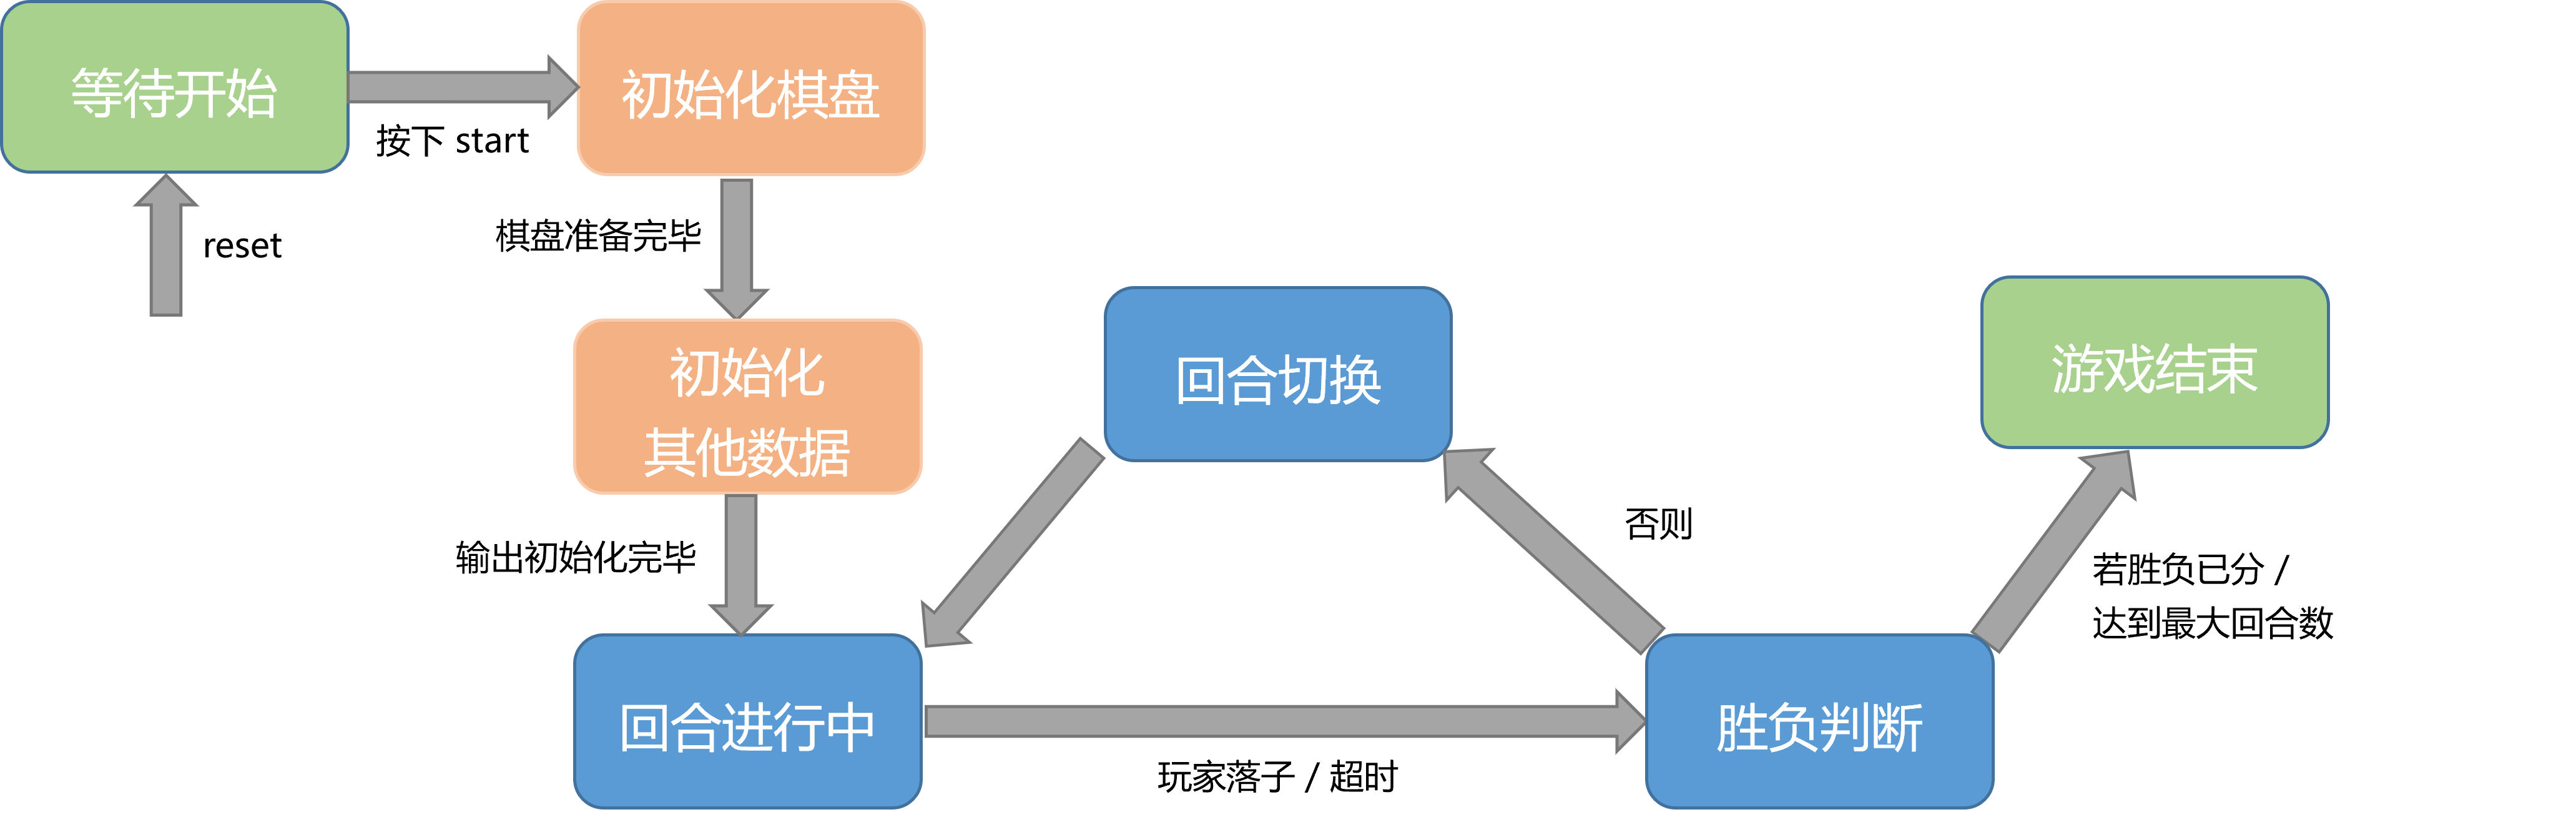
\includegraphics[scale=0.55]{images/states.png}
    \caption{状态转移图}
    \label{fig:state-transfer}
\end{figure}

各状态下,游戏控制器执行的任务以及状态转移见第 \ref{subsubsection:logic} 节。


\subsubsection{游戏运行逻辑} \label{subsubsection:logic}
游戏逻辑部分(以及操作读取器)的逻辑封装在一个 \texttt{always\_ff} 块中,代码如下(行号即为 \texttt{Game\_Controller.sv} 中的行号)。

\begin{lstlisting}[
    language=Verilog,
    numbers=left,
    frame=single,           % 添加边框
    basicstyle=\fontsize{10}{12}\selectfont, % 设置全局字号
    lineskip=4pt,           % 设置行距
    tabsize=4,              % 设置制表符的宽度为4个空格
    xleftmargin=15pt,       % 设置左侧缩进的距离为15pt
    firstnumber=175,
    caption={游戏逻辑部分顶层 \texttt{always} 块} % 标题
] 
// 与键盘输入模块交互+游戏逻辑部分 顶层 always 块
always_ff @ (posedge clock, posedge reset) begin
    if (reset) begin
        state <= READY;
    end else begin
        // 如果键盘输入模块有新数据,那么本周期读取数据,不运行游戏逻辑
        if (keyboard_ready) begin
            // 缓存一次未结算的操作
            if (keyboard_data <= 'b101) begin
                operation <= Operation'(keyboard_data);
            end
            // 并给键盘处理模块返回读取已完成的信号
            keyboard_read_fin <= 'b1;
        // 否则,本周期运行游戏逻辑
        end else begin
            keyboard_read_fin <= 'b0;
            casez (state)
                READY:              ready();
                LOAD_INIT_BOARD:    load_init_board();
                ABOUT_TO_START:     about_to_start();
                IN_ROUND:           in_round();
                CHECK_WIN:          check_win();
                ROUND_SWITCH:       round_switch();
                GAME_OVER:          ;
                default: ; // assert 这种情况不应出现
            endcase
        end
    end
end
\end{lstlisting}

可以看出,如果键盘输入模块(键盘解码器)有新数据,那么本时钟周期读取数据,不运行游戏逻辑。

否则,
我们将每个状态下对应的需要执行的代码各封装为一个 task,各个 task 执行的任务如下:
\begin{itemize}
    \item \texttt{ready}:检查此时的 start 按钮是否处于按下状态。若是,重置棋盘信息,并准备开始载入初始棋盘,然后转移到 LOAD\_INIT\_BOARD 状态。
    \item \texttt{load\_init\_board}:加载初始棋盘数据。在加载完成之前,将保持在 \texttt{LOAD\_INIT\_BOARD} 状态;加载完成之后,转到 \texttt{ABOUT\_TO\_START} 状态,初始化其他游戏数据。
    \item \texttt{about\_to\_start}:完成开始游戏前的其它准备(操作队列初始化为空、随机产生先手玩家、将光标放置在先手玩家的王城等),然后转到 \texttt{IN\_ROUND} 状态,准备开始游戏。
    \item \texttt{in\_round}:回合内的游戏逻辑。如果已超时,状态直接转移到  \texttt{CHECK\_WIN} ;否则,如果当前有尚未结算的操作,那么结算一次操作、将操作队列清空,然后转移到 \texttt{CHECK\_WIN}
    \item \texttt{check\_win}:进行胜负判断。如果某方王城位置归属不再是自己,游戏结束;否则,如果已经达到回合上限,游戏结束,并根据王城兵力决定胜负;否则,游戏继续,进行回合切换。若游戏结束,转移到 \texttt{GAME\_OVER} 状态;否则,转移到 \texttt{ROUND\_SWITCH} 。
    \item \texttt{round\_switch}:进行回合切换。更新光标位置、回合数、当前玩家等数据。每1回合或每 16 回合结束时,增加兵力。状态切换到 \texttt{IN\_ROUND}。
\end{itemize}


% 以上游戏运行逻辑可以概括为以下框图。
% \begin{figure}[H]
%     \centering
%     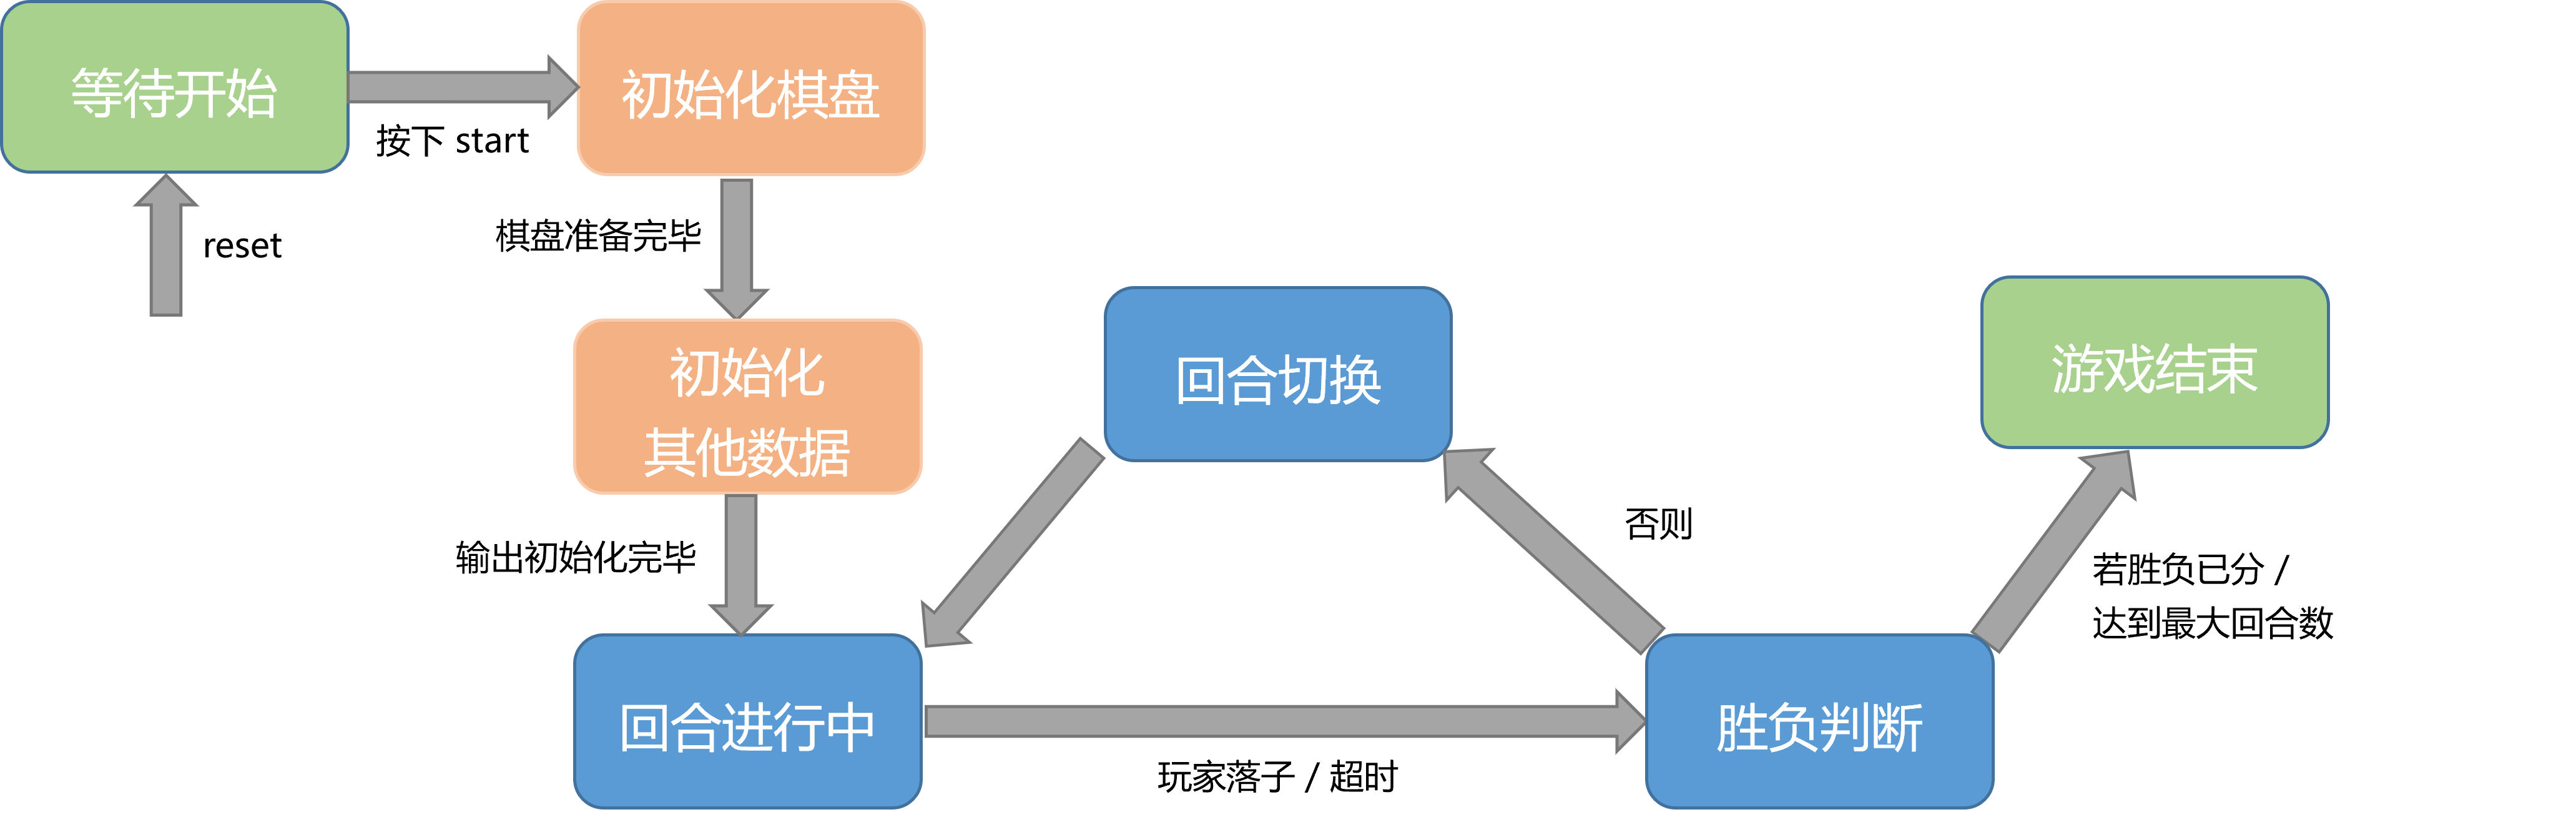
\includegraphics[scale=0.55]{images/states.png}
%     \caption{游戏运行逻辑框图}
%     \label{fig:logic}
% \end{figure}

\subsubsection{随机初始棋盘}
简便起见,在本实现中,随机初始棋盘的实现方式如下。先使用 Python 脚本生成随机棋盘库(容量为 128)。在游戏开始时,玩家先按下 reset ,此时重置一个高频率(50 MHz)的循环计数器,当玩家按下另一个键(clock\_btn)时,即选定一个随机数,然后加载对应的初始地图。

随机先手玩家同样采用类似的抽签方式产生,唯一区别是使用的时钟频率为 100 MHz,这样可以保证每张地图不与某一方玩家绑定,而是在地图选定之后,双方各有 50\% 的概率先手。

生成初始棋盘的脚本为 \texttt{utils/random\_boards.py} 。使用方式见 \texttt{utils/README.md}。该脚本以运行时间为种子,生成随机初始棋盘。

生成的棋盘保证:
\begin{itemize}
    \item 布局合理
        \begin{itemize}
            \item 每个棋盘不超过 32 个“特殊元素”(其中恰有 2 个王城),NPC 特殊元素(山地、空地)不超过 30 个。其余元素均为 NPC 空地。
            \item NPC 特殊元素(山地、空地)的比例均在 35\% 与 65\% 之间。
            \item 双方王城的距离充分大(曼哈顿距离不小于 12)且不在边缘。
            \item 每个王城附近 $3\times 3$ 内至少有 1 个 NPC 城市。
        \end{itemize}
    \item 游戏可终止
        \begin{itemize}
            \item  双方王城之间是连通的,即存在一条连接双方王城的、不经过任何山的路径。
        \end{itemize}
\end{itemize}

\subsubsection{随机初始棋盘数据结构}

脚本生成的初始棋盘为若干个 word(字),每连续的 32 个 word 为 1 张初始棋盘的数据。每个word表示一个“特殊元素”,大小为 10 bit。
\begin{itemize}
    \item 该元素横坐标(h坐标):4位
    \item 该元素纵坐标(v坐标):4位
    \item 该元素类型:2位
        \begin{itemize}
            \item 山地:00
            \item NPC城市:01
            \item 红方王城:10
            \item 蓝方王城:11
        \end{itemize}
\end{itemize}

若特殊元素数目不足32,剩下的word的 (h, v) 记为(0xF, 0xF),表示该word仅用于填充至32个word(也相当于表示该格为NPC普通领地)。


\subsubsection{模块接口}
下面为模块接口:

\begin{lstlisting}[
    language=Verilog,
    numbers=left,
    frame=single,           % 添加边框
    basicstyle=\fontsize{10}{12}\selectfont, % 设置全局字号
    lineskip=4pt,           % 设置行距
    tabsize=4,              % 设置制表符的宽度为4个空格
    xleftmargin=15pt,       % 设置左侧缩进的距离为15pt
    % firstnumber=174,
    caption={游戏逻辑部分模块接口(仅用于测试的输出略去)} % 标题
]
module Game_Controller
#(parameter VGA_WIDTH            = 0, 
            BORAD_WIDTH          = 10, 
            LOG2_BORAD_WIDTH     = 4, 
            MAX_PLAYER_CNT       = 7, 
            LOG2_MAX_PLAYER_CNT  = 3, 
            LOG2_PIECE_TYPE_CNT  = 2, 
            LOG2_MAX_TROOP       = 9, 
            LOG2_MAX_ROUND       = 12,
            ROUND_LIMIT          = 999,
            LOG2_MAX_CURSOR_TYPE = 2,
            MAX_STEP_TIME        = 15,
            LOG2_MAX_STEP_TIME   = 5,
            MAX_RANDOM_BOARD     = 128) (
    //// input
    input wire                    clock,
    input wire                    clock_random_first_player,
    input wire                    start,              // 游戏开始
    input wire                    reset,
    // 与 Keyboard_Decoder 交互:获取键盘操作信号 
    input wire                    keyboard_ready,
    input wire [2: 0]             keyboard_data,

    // 与 Screen_Controller(的 vga 模块)交互: 获取当前的横纵坐标
    input wire [VGA_WIDTH - 1: 0] hdata,
    input wire [VGA_WIDTH - 1: 0] vdata,

    //// output
    // 与 Keyboard_Decoder 交互:输出键盘操作已被读取的信号
    output wire                   keyboard_read_fin,  
    // 游戏逻辑生成的图像
    output wire [7: 0]            gen_red,
    output wire [7: 0]            gen_green,
    output wire [7: 0]            gen_blue,
    output wire                   use_gen
);
\end{lstlisting}

输入:
\begin{itemize}
    \item \texttt{clock}:输入时钟,为 $50 \text{MHz}$ 的时钟。
    \item \texttt{clock\_random\_first\_player}:$100 \text{MHz}$ 的时钟,仅用于抽签产生随机先手玩家。
    \item \texttt{start}:游戏开始按键信号。
    \item \texttt{reset}:重置信号。连接 reset 按钮,该信号为 1 时,游戏会重置到 \texttt{READY} 状态。
    \item \texttt{keyboard\_ready}, \texttt{keyboard\_data}:与键盘解码器交互的信号,参见第 \ref{subsubsection:interact-input-logic} 节。
    \item \texttt{hdata}, \texttt{vdata}:与输出控制器交互的信号,参见第 \ref{subsubsection:interact-logic-output} 节。
\end{itemize}

输出:
\begin{itemize}
    \item \texttt{keyboard\_read\_fin}:与键盘解码器交互的信号,参见第 \ref{subsubsection:interact-input-logic} 节。
    \item \texttt{gen\_red}, \texttt{gen\_blue}, \texttt{gen\_green}, \texttt{use\_gen}:与输出控制器交互的信号,参见第 \ref{subsubsection:interact-logic-output} 节。
\end{itemize}


\subsection{游戏画面绘制}
项目中与该部分对应的 module 为 \texttt{Game\_Controller}模块(代码的后半部分),\texttt{Background\_Painter}模块,\texttt{Number\_Transfer}模块,和\texttt{Number\_Choose}模块。

\subsubsection{实现细节}
本项目存储的全部图片素材都以mif格式存储在片内RAM中,对每张图片素材使用一个RAM ip核,把像素位置转换为一维地址后传入ip核,从而读出对应像素应绘制的RGB值。使用的图片素材包括所有特殊格子类型(不同归属的 城市/王城/山地)、数字0-9(分为大小版本,大版本用作回合数、倒计时显示,小版本用作兵力显示)和文字(包括“50\%”字样、WINNER 和 DRAW)。

游戏画面绘制主逻辑在\texttt{Game\_Controller}代码的后半部分实现,读入游戏逻辑部分保存的局面信息,接收由显示控制器部分VGA扫描传来的当前像素横纵坐标,根据局面选择显示的内容。绘制内容整体分为两种,即背景和游戏内容,背景部分通过\texttt{Background\_Painter}模块直接操控RGB值绘制($10\times 10$ 的黑框灰底棋盘),游戏内容部分由\texttt{Game\_Controller}绘制,根据上述信息绘制数字、文字、特殊格子,并进行数据选择,判断该像素使用背景还是游戏内容,把选择信息和显示数据传给 \texttt{Screen\_Controller}。

\texttt{Number\_Transfer}模块对于读入的数字打表作取模运算,将三位数拆分为百位、十位、个位,用于分别显示。该模块由\texttt{Game\_Controller}调用。

\texttt{Number\_Choose}模块读入当前像素,打表取模转换为RAM地址,根据读入的个位、十位、百位作数据选择,将最后确定的数字显示数据(RGB)传给\texttt{Game\_Controller}。该模块由\texttt{Game\_Controller}调用。

\subsubsection{模块接口}
下面为模块接口:
\begin{lstlisting}[
    language=Verilog,
    numbers=left,
    frame=single,           % 添加边框
    basicstyle=\fontsize{12}{12}\selectfont, % 设置全局字号
    lineskip=4pt,           % 设置行距
    tabsize=4,              % 设置制表符的宽度为4个空格
    xleftmargin=15pt,       % 设置左侧缩进的距离为15pt
    caption={\texttt{Background\_Painter}源代码} % 标题
] 
module Background_Painter
# (parameter VGA_WIDTH = 0) (
	input  wire[VGA_WIDTH - 1:0] hdata,
	input  wire[VGA_WIDTH - 1:0] vdata,
	output wire[7:0] video_red,
	output wire[7:0] video_green,
	output wire[7:0] video_blue
);
\end{lstlisting}

输入:
\begin{itemize}
    \item \texttt{hdata}:当前像素VGA扫描横坐标
    \item \texttt{vdata}:当前像素VGA扫描纵坐标
\end{itemize}

输出:
\begin{itemize}
    \item \texttt{video\_red}:当前像素背景r值
    \item \texttt{video\_green}:当前像素背景g值
    \item \texttt{video\_blue}:当前像素背景b值
\end{itemize}

\begin{lstlisting}[
    language=Verilog,
    numbers=left,
    frame=single,           % 添加边框
    basicstyle=\fontsize{12}{12}\selectfont, % 设置全局字号
    lineskip=4pt,           % 设置行距
    tabsize=4,              % 设置制表符的宽度为4个空格
    xleftmargin=15pt,       % 设置左侧缩进的距离为15pt
    caption={\texttt{Number\_Choose}源代码} % 标题
] 
module Number_Choose
#(parameter VGA_WIDTH            = 0,
			LOG2_BORAD_WIDTH     = 4)
(
	input wire[VGA_WIDTH-1:0] 				hdata,
	input wire[VGA_WIDTH-1:0]				vdata,
	input wire[3:0]							cur_ones,
	input wire[3:0]							cur_tens,
	input wire[3:0]							cur_hundreds,
	input wire[3:0]							big_ones,
	input wire[3:0]							big_tens,
	input wire[3:0]							big_hundreds,
	input									clock,
    output wire [VGA_WIDTH - 1: 0]          vdata_to_ram,
    output wire [VGA_WIDTH - 1: 0]          hdata_to_ram,
	output wire[31:0]						bignumberdata,
	output wire[LOG2_BORAD_WIDTH - 1:0]		cur_h,
	output wire[LOG2_BORAD_WIDTH - 1:0]		cur_v,
	output wire[31:0]						numberdata
);
\end{lstlisting}

输入:
\begin{itemize}
    \item \texttt{video\_red}:当前像素背景r值
    \item \texttt{video\_green}:当前像素背景g值
    \item \texttt{video\_blue}:当前像素背景b值
    \item \texttt{cur\_ones}:当前格兵力数字个位 
    \item \texttt{cur\_tens}:当前格兵力数字十位 
    \item \texttt{cur\_hundreds}:当前格兵力数字百位 
    \item \texttt{cur\_ones}:当前大数字(回合或倒计时)个位 
    \item \texttt{cur\_tens}:当前大数字十位 
    \item \texttt{cur\_hundreds}:当前大数字百位 
    \item \texttt{clock}:输入时钟,为$50 \text{MHz}$ 的游戏逻辑部分主时钟
\end{itemize}


输出:
\begin{itemize}
    \item \texttt{vdata\_to\_ram}:对40取模后的纵坐标,用于计算RAM地址
    \item \texttt{hdata\_to\_ram}:对40取模后的横坐标,用于计算RAM地址
    \item \texttt{bignumberdata}:从RAM中读取的大数字像素RGB值
    \item \texttt{numberdata}:从RAM中读取的兵力数字像素RGB值
    \item \texttt{cur\_h}:当前像素所在棋盘格横坐标
    \item \texttt{cur\_v}:当前像素所在棋盘格纵坐标
\end{itemize}

\begin{lstlisting}[
    language=Verilog,
    numbers=left,
    frame=single,           % 添加边框
    basicstyle=\fontsize{12}{12}\selectfont, % 设置全局字号
    lineskip=4pt,           % 设置行距
    tabsize=4,              % 设置制表符的宽度为4个空格
    xleftmargin=15pt,       % 设置左侧缩进的距离为15pt
    caption={\texttt{Number\_Transfer}源代码} % 标题
] 
module Number_Transfer
#(parameter BIT = 9)(
	input wire [BIT-1:0] number,
	output wire [3:0] ones,
	output wire [3:0] tens,
	output wire [3:0] hundreds
);
\end{lstlisting}

输入:
\begin{itemize}
    \item \texttt{number}:传入的三位十进制数字,用于转换为个位、十位、百位
\end{itemize}

输出:
\begin{itemize}
    \item \texttt{ones}:个位
    \item \texttt{tens}:十位
    \item \texttt{hundreds}:百位
\end{itemize}


\subsection{显示控制器}
项目中与该部分对应的 module 为 \texttt{Screen\_Controller}。
\subsubsection{实现细节}
该部分首先调用VGA控制器,扫描生成行列坐标,传入\texttt{Game\_Controller}。然后分别读入\texttt{Game\_Controller}生成的画面数据和\texttt{Background\_Painter}生成的背景画面数据,根据\texttt{Game\_Controller}传入的数据选择信息,最终确定向外输出的画面RGB值。

\subsubsection{模块接口}
\begin{lstlisting}[
    language=Verilog,
    numbers=left,
    frame=single,           % 添加边框
    basicstyle=\fontsize{12}{12}\selectfont, % 设置全局字号
    lineskip=4pt,           % 设置行距
    tabsize=4,              % 设置制表符的宽度为4个空格
    xleftmargin=15pt,       % 设置左侧缩进的距离为15pt
    caption={\texttt{Screen\_Controller}源代码} % 标题
] 
module Screen_Controller
#(parameter VGA_WIDTH = 0, HSIZE = 0, HFP = 0, HSP = 0, 
HMAX = 0, VSIZE = 0, VFP = 0, VSP = 0, VMAX = 0, HSPP = 0, 
VSPP = 0)
(
    // 时钟、复位
    input  wire clk_vga,             // vga 输入时钟 (25M)
    input  wire reset_n,             // 上电复位信号,低有效
    // 游戏逻辑生成的图像
    input  wire [7: 0] gen_red,
    input  wire [7: 0] gen_green,
    input  wire [7: 0] gen_blue,
    input  wire        use_gen,      // 当前像素是使用游戏
    逻辑生成的图像(1)还是背景图(0)

    // 当前横纵坐标
    output wire [VGA_WIDTH - 1: 0] hdata_o,
    output wire [VGA_WIDTH - 1: 0] vdata_o,

    // HDMI 图像输出
    // '_O' 后缀表示该输出将直接接到 mod_top 的对应输出
    output wire [7: 0] video_red_O,   // 红色像素,8位
    output wire [7: 0] video_green_O, // 绿色像素,8位
    output wire [7: 0] video_blue_O,  // 蓝色像素,8位
    output wire        video_hsync_O, // 行同步信号
    output wire        video_vsync_O, // 场同步信号
    output wire        video_clk_O,   // 像素时钟输出
    output wire        video_de_O     // 行数据有效信号,
    用于区分消隐区

);
\end{lstlisting}

输入:
\begin{itemize}
    \item \texttt{clk\_vga}:vga输入时钟,为$25 \text{MHZ}$
    \item \texttt{reset\_n}:复位信号,低有效
    \item \texttt{gen\_red}:\texttt{Game\_Controller}绘制的R值
    \item \texttt{gen\_green}:\texttt{Game\_Controller}绘制的G值
    \item \texttt{gen\_blue}:\texttt{Game\_Controller}绘制的B值
    \item \texttt{use\_gen}:判断当前像素使用有游戏逻辑生成的画面还是背景
\end{itemize}

输出:
\begin{itemize}
    \item \texttt{hdata\_o}:vga扫描得到的当前横坐标
    \item \texttt{vdata\_o}:vga扫描得到的当前纵坐标
    \item \texttt{video\_red\_O}:输出到屏幕的R值
    \item \texttt{video\_green\_O}:输出到屏幕的G值
    \item \texttt{video\_blue\_O}:输出到屏幕的B值
    \item \texttt{video\_hsync\_O}:行同步(水平同步)信号
    \item \texttt{video\_vsync\_O}:场同步(垂直同步)信号
    \item \texttt{video\_clk\_O}:像素时钟输出
    \item \texttt{video\_de\_O}:行数据有效信号,用于区分消隐区
\end{itemize}

\section{遇到的困难及解决}

\subsection{初始棋盘信息不正确的问题}
一开始初始棋盘写成 MIF 文件,存在RAM里,用 ip 核读取。但少数情况下读取的少部分数据有问题,猜测可能是 RAM 内存在“噪点”或其它异常。将初始棋盘改成直接用 \texttt{localparam} 写在程序里(打表),可以正常加载初始棋盘。

\subsection{SV 语言特性}
\subsubsection{时序逻辑块中的寄存器赋值问题}

一个寄存器在一个 \texttt{always\_ff} 块中只能赋值一次。如果有多次赋值,那么除最后一个赋值语句之外的语句都将被覆盖。

对于本游戏,在每一回合结束时,既需要结算玩家操作引起的兵力变化,又需要结算兵力的自然增长。为了避免实现代码过于复杂且混乱,我们将这两个部分分离,具体而言即增加 \texttt{ROUND\_SWITCH} 状态,用于结算兵力的自然增长,将两部分兵力变化分开在两个周期内进行。这样同时也让代码的模块化更佳。

\subsubsection{组合逻辑块中的赋值问题}
每个 \texttt{always\_comb}块必须覆盖 \texttt{if} 的所有情况,同时在每种情况下都为变量赋值,否则无法编译。这与平时软件语言的惯例不同,曾导致花费了大量时间来找编译不通过的问题

\subsubsection{运算符语法问题}
Verilog 具有自己的运算语法,尤其是运算符优先级的问题,如移位运算在加法运算之后,这一度导致我们无法正确读取棋盘数据(因为地址运算错误),在查询资料后修改解决。

\subsection{时序问题}
初期,我们选用50MHz时钟用于 $800\times600@75 \, \text{Hz}
$ VGA 显示,100MHz时钟用于游戏内部逻辑运算,发现在早期没有太多逻辑运算时可以维持,但只要增加逻辑就会发生时序报错,画面无法正常渲染。为了避免时序要求不满足的问题,我们采取了两个措施:

\textcircled{1}内部逻辑提速:考虑到复杂性问题,我们将所有的除法(包括取模)和部分乘法用打表实现,这在初期显著提高了性能。

\textcircled{2}更换时钟:在逻辑运算大量增加后,我们意识到原有的时钟频率不能支持这个规模的运算,决定更改时钟,同时修改VGA以适配,选用25MHz时钟用于 $640\times480@60 \, \text{Hz}
$ VGA 显示,50MHz时钟用于游戏内部逻辑运算。调整后,项目时序报错问题得到解决,运行时具有较高的稳定性。
\section{实验总结}
\subsection{FPGA 资源利用情况}

本项目共占用 FPGA 逻辑资源 21\%,内存资源 48\%,均在合理范围内。

\begin{figure}[H]
    \centering
    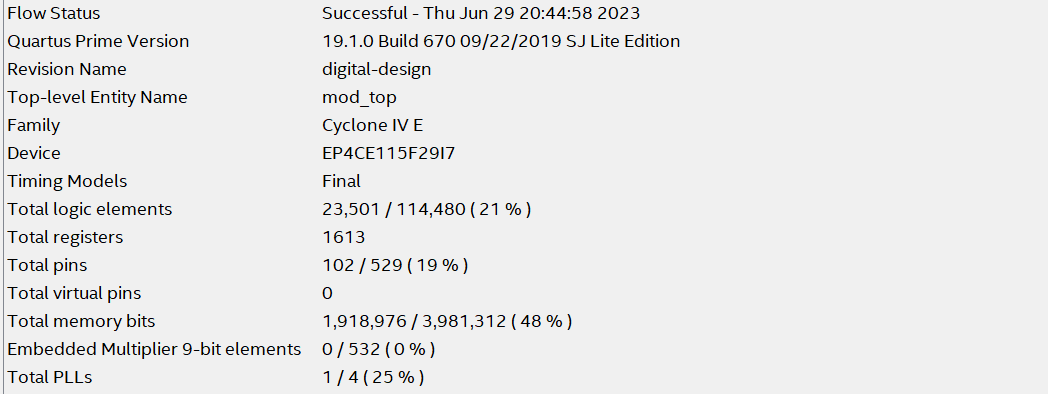
\includegraphics[scale=0.82]{images/compile_result.png}
    \caption{FPGA 资源利用情况}
    \label{fig:compile_result}
\end{figure}


% \subsection{未来工作}
% 这部分保留还是去掉?

\subsection{总结与心得}
本次项目中,我们预先设计了较为完整的文件框架,将项目各功能分开封装处理,提前写好模块接口,同时维护了比较细节的 README 文件,这帮助我们在开发时保持有序,大大提高了开发效率。

实际开发时,由于本学期课业紧张,我们并没有太多富余的时间,这使得我们工期一度吃紧。这值得我们在时间分配问题上作出反思,日后做到合理地配置,而非逐个赶工。不过受益于良好的项目框架管理,且我们及时调整了项目计划目标,砍掉了一些过于复杂的初期设想,最后还是很好地完成了预期的游戏功能。

开发过程中,我们保障了比较充足的实验室测试时间,尤其是输出部分,做到随写、随测、随修(debug),同时及时获取进度快的同学与助教老师的帮助,这些都帮助了我们快速、可靠地完成项目。

此外,这次开发使我们亲身体会了硬件语言的特殊性,如时序分析、时序逻辑特殊语法、组合逻辑必须覆盖所有情况等要求,这帮助我们拓宽了对编程语言的认识,同时深化了对课上所学数字逻辑的理解。

最后,感谢不辞辛劳的老师和助教的鼓励与帮助。

\end{document}
